\begin{table}
  \centering
  \setlength{\tabcolsep}{5pt}
  \begin{tabular}{lrrr}
    \toprule
    \bf \multirow{2}{*}{Name} & \bf Contracts & \bf Vulnerabilities & \bf Ether at stake\\
                              & \bf analyzed & \bf found & {\small at time of report} \\
    \midrule
    Oyente & 19,366 & 7,527 & 1,287,032\\
    Zeus & 1,120 & 861 & 671,188\\
    Maian & NA & 2,691 & 15.59 \\
    Securify & 29,694 & 9,185 & 724,306\\
    MadMax & 91,800 & 6,039 & 1,114,958\\
    teEther & 784,344 & 1,532 & 1.55\\
    \bottomrule
  \end{tabular}
  \caption{Summary of the contracts in our dataset.}
  \label{fig:dataset-stats}
\end{table}

\subsection{Dataset}
\label{sec:datasets}
In this section, we analyze the vulnerable contracts reported by the following~\PapersAnalyzed academic papers:~\cite{Luu2016a},~\cite{DBLP:conf/ndss/KalraGDS18},~\cite{Nikolic2018a},~\cite{Tsankov2018},~\cite{Grech2018} and~\cite{Krupp2018}. To collect information about the addresses analyzed and the vulnerabilities found, we reached out to the authors of the different papers.

Oyente~\cite{Luu2016a} data was publicly available~\cite{oyente-benchmarks}. The authors of the other papers were kind enough to provide us with their dataset. We received all the replies within less than a week of contacting the authors.

We also reached out to the authors of~\cite{Tikhomirov2017},~\cite{Jiang2018} and~\cite{Brent2018} but could not obtain their dataset, which is why we left these papers out of our analysis.

Our dataset is comprised of a total of \empirical{821,219} contracts, of which \VulnerableContracts contracts have been flagged as vulnerable to at least one of the~\VulnTypes vulnerabilities described in Section~\ref{sec:background}. Although we received the data directly from the authors, the numbers of contracts analyzed usually did not match the data reported in the papers, which we show in Figure~\ref{fig:prior-results}. We believe the two main results for this are: authors improving their tools after the publication and authors not including duplicated contracts in their data they provided us. Therefore, we present the numbers in our dataset, as well as the Ether at stake for vulnerable contracts in Figure~\ref{fig:dataset-stats}. The Ether at stake is computed by summing the balance of all the contracts flagged vulnerable. We use the balance at the time at which each paper was published rather than the current one, as it gives a better sense of the amount of Ether which could potentially have been exploited.

\begin{table}[tb]
  \begin{subfigure}{0.48\columnwidth}
    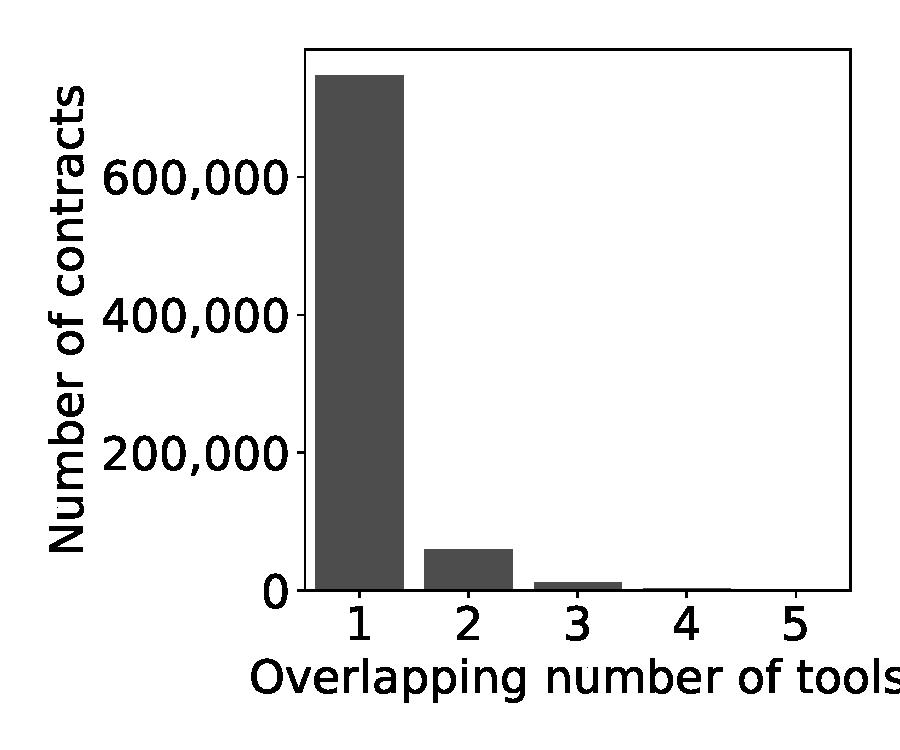
\includegraphics[width=\textwidth]{./5a-smart-contract-security/figures/overlap-analyzed.pdf}
    \caption{Overlapping contracts\\analyzed.}
    \label{fig:all-overlap}
  \end{subfigure}
  \begin{subfigure}{0.48\columnwidth}
    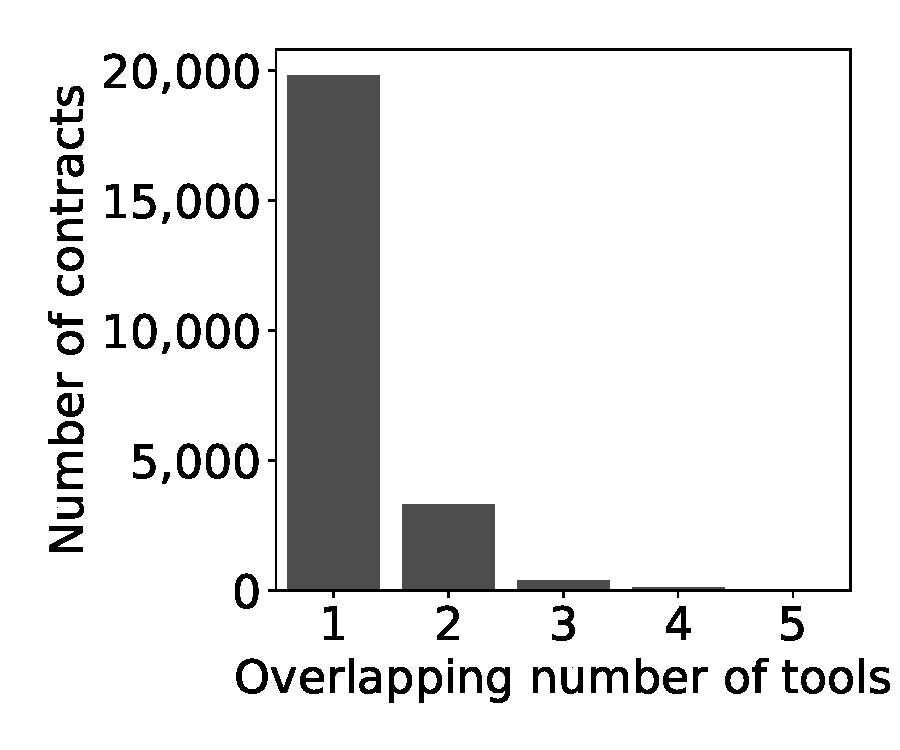
\includegraphics[width=\textwidth]{./5a-smart-contract-security/figures/overlap-vulnerable.pdf}
    \caption{Overlapping vulnerabilities\\\centering flagged.}
    \label{fig:vulnerable-overlap}
  \end{subfigure}
  \caption{Histograms that show the overlap in the contracts analyzed and flagged by examined tools.}
\label{fig:hist-per-tool}
\end{table}

\begin{figure}[tb]
  \setlength{\tabcolsep}{2pt}
  \centering
  \begin{tabular}{lrrrr}
    \toprule
    \bf Tools & \bf Total & \bf Agreed & \bf Disagreed & \bf \% agreement\\
    \midrule
    Oyente/Securify & 774 & 185 & 589 & 23.9\%\\
    Oyente/Zeus & 104 & 3 & 101 & 2.88\%\\
    Zeus/Securify & 108 & 2 & 106 & 1.85\%\\
    \bottomrule
  \end{tabular}
  \caption{Agreement among tools for re-entrancy analysis.}
  \label{fig:reentrancy-agreement}
\end{figure}

\begin{table}
  \centering
  \setlength{\tabcolsep}{2pt}
  \small
  \begin{tabular}{lllllll}
    \toprule
    & \bf Oyente & \bf ZEUS & \bf Securify & \bf MadMax & \bf Maian & \bf teEther\\
    \midrule
    \bf \vre & re-entrancy & re-entrancy & no writes after call & --- & --- & ---\\
    \hline
    \bf \vue & callstack & unchecked send & handled exceptions & --- & --- & ---\\
    \hline
    \bf \vto & concurrency & tx order dependency & tx ordering dependency & --- & --- & ---\\
    \hline
    \bf \vle & --- & failed send & Ether liquidity & unbounded op & greedy & ---\\
    & & & & wallet griefing\\
    \hline
    \bf \vio & --- & integer overflow & --- & integer overflows & --- & --- \\
    \hline
    \bf \vua & --- & integer overflow & --- & integer overflows & prodigal & exploitable\\
    \bottomrule
  \end{tabular}
  \caption{Mapping of the different vulnerabilities analyzed.}
  \label{fig:vuln-mapping}
\end{table}

\point{Taxonomy}
Rather than reusing existing smart contracts vulnerabilities taxonomies~\cite{Atzei2017} as-is, we adapt it to fit the vulnerabilities analyzed by the tools in our dataset. We do not cover vulnerabilities not analyzed by at least \empirical{two} of the \PapersAnalyzed tools. We settle on the~\VulnTypes types of vulnerabilities described in Section~\ref{sec:background}: re-entrancy (\vre), unhandled exception (\vue), locked Ether (\vle), transaction order dependency (\vto), integer overflows (\vio) and unrestricted actions (\vua). As the papers we survey use different terms and slightly different definitions for each of these vulnerabilities, we map the relevant vulnerabilities to one of the \VulnTypes types of vulnerabilities we analyze. We show how we mapped these vulnerabilities in Figure~\ref{fig:vuln-mapping}.

% \point{Excluded data}
% We exclude teEther~\cite{Krupp2018} and Maian~\cite{Nikolic2018a} from our analysis for two reasons. First, the amount of Ether at stake is too low to make an impact on our final results. The amount of Ether at stake for both tools combined represent a total of \empirical{14.89} Ether, which is \emph{six orders of magnitude} less than the total. Second, for the classes of vulnerabilities treated by these tools, it is almost impossible to assess if these vulnerabilities have been exploited or not. Indeed, for a vulnerability such as being able to destruct the contract, there is no general way of knowing if the person who performed such a call should have been allowed to do so. Given this lack of reliability and the very low amount of money at stake, we decided to keep this data out of further analysis.

\point{Overlapping vulnerabilities}
In this subsection, we first check how much overlap there is between contracts in our dataset: how many contracts have been analyzed by multiple tools and how many contracts were flagged vulnerable by multiple tools.
We note that most papers, except for~\cite{Luu2016a}, are written around the same period. We find that~\empirical{73,627} out of~\empirical{821,219} contracts have been analyzed by at least two of the tools but only~\empirical{13,751} by at least three tools.
In Figure~\ref{fig:all-overlap}, we show a histogram of how many different tools analyze a single contract. In Figure~\ref{fig:vulnerable-overlap}, we show the number of tools which flag a single contract as vulnerable to any of the analyzed vulnerability. The overlap for both the analyzed and the vulnerable contracts is relatively small. We assume one of the reasons is that some tools work on Solidity code~\cite{DBLP:conf/ndss/KalraGDS18} while other tools work on EVM bytecode~\cite{Tsankov2018,Luu2016a}, making the population of contracts available different among tools.

We also find a lot of contradiction in the analysis of the different tools.
We choose re-entrancy to illustrate this point, as it is supported by three of the tools we analyze. In Figure~\ref{fig:reentrancy-agreement}, we show the agreement between the three tools supporting re-entrancy detection. The \emph{Total} column shows the total number of contracts analyzed by both tools in the \emph{Tools} column and flagged by at least one of them as vulnerable to re-entrancy. Oyente and Securify agree on only~\empirical{23\%} of the contracts, while Zeus does not seem to agree with any of the other tools.
This reflects the difficulty of building static analysis tools targeted at the EVM. While we are not trying to evaluate the different tools' performance, this gives us yet another motivation to find out the impact of the reported vulnerabilities.
